\documentclass[12pt]{article}
\usepackage{amsmath}
\usepackage{amsfonts}
\usepackage{mathrsfs}
\usepackage{lscape}
\usepackage{listings}
\usepackage{graphicx} % Allows for importing of figures
\usepackage{color} % Allows for fonts to be colored
\usepackage{comment} % Allows for comments to be made
\usepackage{accents} % Allows for accents to be made above and below text
%\usepackage{undertilde} % Allows for under tildes to take place for vectors and tensors
\usepackage[table]{xcolor}
\usepackage{array,ragged2e}
\usepackage{hyperref}
\usepackage{framed} % Allows boxes to encase equations and such
\usepackage{subcaption} % Allows for figures to be side-by-side
\usepackage{float} % Allows for images to not float in the document
\usepackage{booktabs}
%\usepackage[margin=0.75in]{geometry}
\usepackage[final]{pdfpages}
\usepackage{enumitem}
\usepackage[section]{placeins}

%%%%%%%%%%%%%%%%%%%%%%%%%  Function used to generate vectors and tensors %%%%%%%%%
\usepackage{stackengine}
\stackMath
\newcommand\tensor[2][1]{%
	\def\useanchorwidth{T}%
	\ifnum#1>1%
	\stackunder[0pt]{\tensor[\numexpr#1-1\relax]{#2}}{\scriptscriptstyle \sim}%
	\else%
	\stackunder[1pt]{#2}{\scriptscriptstyle \sim}%
	\fi%
}
%%%%%%%%%%%%%%%%%%%

\definecolor{mygrey}{rgb}{0.97,0.98,0.99}
\definecolor{codeblue}{rgb}{.2,0,1}
\definecolor{codered}{rgb}{1,0,0}
\definecolor{codegreen}{rgb}{0.3,0.33,0.12}
\definecolor{codegray}{rgb}{0.5,0.5,0.5}
\definecolor{codepurple}{rgb}{0.55,0.0,0.55}
\definecolor{codecyan}{rgb}{0.0,.4,.4}

\lstdefinestyle{mystyle}{
	backgroundcolor=\color{mygrey},   
	commentstyle=\color{codegreen},
	keywordstyle=\color{codeblue},
	stringstyle=\color{codepurple},
	numberstyle=\tiny\color{codegray},
	basicstyle=\footnotesize,
	breakatwhitespace=false,         
	breaklines=true,                 
	captionpos=b,                    
	keepspaces=true, 
	numbers=left,                    
	numbersep=5pt,                  
	showspaces=false,                
	showstringspaces=false,
	showtabs=false,                  
	tabsize=2
}
\lstset{style=mystyle}

\lstset{language=Matlab,backgroundcolor=\color{mygrey}}
\usepackage{lastpage}
\usepackage{fancyhdr}
\pagestyle{fancy}
%\lhead{\large{Nik Benko, John Callaway, Nick Dorsett, Martin Raming}} 
%\chead{\large{\textbf{ME EN 6960: Lab 1}}}
%\rhead{\today}
\cfoot{[\thepage\ of \pageref{LastPage}]}
\fancyheadoffset{.5cm}
\setlength{\parindent}{0cm}
\usepackage[left=.5in, right=0.50in, top=1.00in,bottom=1.00in]{geometry}
\usepackage{microtype} 
%%%%%%%%%%%%%%%%%%%%%%%%%%%%%%%%%%%%%%%%%%%%%%%%%%%%%%%%%%%%%%%%%%%%%%%%%%


\begin{document}
\title{ Experimental Determination of Composite Stacking Sequence Using Four Point Bend Test\\ \normalsize{ME EN 6960}}
\author{Nik Benko, John Callaway, Nick Dorsett, Martin Raming}
\maketitle
\begin{abstract} %Martin
	There are several different techniques to determine ply orientations within a composite laminate (stacking sequence). In this experiment we utilized laminated plate theory (LPT) with experimental techniques in order to determine the correct stacking sequence of a composite laminate.   We were provided a list of five possible stacking sequences for a composite panel in question. This panel was made of T800-3900 carbon fiber prepreg. LPT can be used to predict either stresses or strains of a composite laminate if given material properties, forces, and a stacking sequence. In this project we utilized LPT to predict strains for loading conditions that would match mechanical testing.  Our mechanical testing consisted of a four-point bend test to induce a known moment in mid-section of our composite specimen. By attaching 3 strain gauges to the mid-section we recorded strains during mechanical testing. We then compared and best matched recorded strains to calculated strains to determine the correct stacking sequence. Verification was done through polishing and visual inspection of a side of the composite laminate.  A four point bend test was used to determine the layup of a composite laminated plate
\end{abstract}

\section{Introduction} %Martin 
Composite materials are currently used in many applications where  a high stiffness to weight ratio is important for design and operations such as in the aerospace and sports industries.  While the idea of using combined materials to improve the capability of a structure has been utilized for thousands of years, use of modern composites like carbon fiber with an epoxy matrix is a relatively new practice.  As the industry first began many questions developed involving  engineering design implications such as failure criteria and material response. The main challenge for modern composites is the orthotropic nature of the material. Modern composite lamina tend to have a significantly larger Young's modulus in the fiber direction compared to the matrix direction.  This orthotropic property is also what makes composites desirable when designing a structure that requires different material responses relative to global orientation. This is done by stacking individual plies in different orientations with respect to each other to create a laminate. The way in which these plies are oriented is also known as a  stacking sequence.

% referance LPT
	
	To analytically understand how a stacking sequence of a laminate responds to a loading condition we turn to laminated plate theory (LPT).  LPT first evolved in the 1950's and 60's.\cite{Gibson} The theory relies on the material properties in the material coordinates system, stacking sequence, and ply thickness to arrive at what is know as the $ABD$ matrix. The $ABD$ matrix can then be used to solve for strains, curvatures and stresses for a given load vector containing forces and moments.  The $ABD$ matrix is  a $6\times 6$ matrix  comprised of 36 components which makes for difficult hand calculations. For this reason it is often convenient to utilize a coding software to perform calculations as was done in this experiment. 
%We utilized two separately written codes in MatLab{\textregistered} for performing LPT calculation off all five stacking sequences to arrive at strains for

	
	LPT has proven to be very useful in design considerations but can be used for other purposes.  In this report we explore the use  and accuracy of LPT to back out a stacking sequence by comparing calculated results to experimental results. The goal of this experiment is to find which of the five unique laminate stacking sequence given  matches the configuration of the specimen in question. In order to get data for comparison we loaded our specimen at intervals in a four-point bend flexure device while recording strains using strain gauges.  We potentially only needed one induced moment but performed several for completeness and accuracy. 
	
	  
	  In this report we start by further expanding on LPT and implications of using the theory.  We then discuss the experimental techniques and performed procedures used to arrive at force induced strains of our specimen. Possible errors and uncertainties  relating to the experiment are then considered at the end of the methods section. Results are presented and discussed in the preceding our conclusion. All figures and tables can be located in section seven. 


\section{Methods}

\subsection{Laminated Plate Theory} %Nik - equations, Nick- Write up

The composite material used in this lab are classified as a specially orthotropic material, meanign that it has two planes of symmetry. Because of this, the material can be defined using 12 total material constants with 5 independent constants. This can then be further reduced to 4 independent constants by assuming the plate is experiencing plane stress conditions. This assumption is valid because the plate is very thin, so all stresses in the z direction will be negligible. The constants used are E{1}, the stiffness in the fiber direction, E{2}, the stiffness 90 degrees from the fiber direction, G{12}, the shear modulus in the 1-2 plane, and \nu{12}, Poisson's ratio defining strain in the 2 direction due to applied force in the 1 direction. These material constants are used in Equation 1 to define the material stiffness matrix [Q]. This [Q] matrix is only appliccable for a single ply with its fibers aligned in the x-direction. Tensor transformations can be used to define the behavior of this single ply in any orientation desired. Equation 2 shows the transformation matrix, [T] of sine and cosine terms used to transform the matrix, and equation 4 is the equation used to actually apply the rotation, generating \bar{Q}, used to denote this transformed stiffness. It is important to note that the Reuter matrix, denoted [R], is used because its factor of 2 is necessary to satisfy tensor rotation rules for shear strain.

These stiffnesses are used to calculate material constants for single plies of material. Laminated Plate Theory (LPT) is used to compute matrices that relate forces, moments, strains, and curvatures over entire laminates. Using LPT requires the assumptions of perfectly bonded plies, plane sections remaining plane during deformation, thin laminates, small midplane displacements and rotations, plane stress conditions, and transverse stresses to be neglected. While these may not be entirely acceptable assumptions to make under all conditions, for most general purposes they are acceptable. These conditions being satisfied, equations 5, 6, and 7 are used to calculate three matricies denoted [A], [B], and [D] based up on the \bar{Q} matrix for each individual ply. These equations are also based on z, which is the distance of each ply interface from the midplane of the laminate. The [A] matrix relates normal forces with normal strains, the [D] matrix relates moments and curvatures, and the [B] matrix relates both normal forces with curvatures and moments with normal strains. Through the combination of these into a single 6x6 matrix, shown in equation 8, laminate response for small deformations can be calculated for any loading scenario.

\subsection{Experimental Techniques} % Martin
\subsubsection{Strain Analysis}
Electrical strain gauges are a commonly used tool in engineering applications to accurately measure axial strain. The essential aspect of a strain gauge is made up of a very thin wire. Since the gauge is bonded to the surface of the material it extends or contracts with the specimen surface.  This elongation or compression of the wires in the strain gauge causes the electrical resistance to change. Strain can then be determined by the fact that material deformation is dependent on material electrical resistivity.  This relationship between resistivity and deformation of the given alloy in a strain gauge is referred to as the gauge factor $(GF)$.  

Electrical strain gauges are essentially a Wheatstone bridge which consists of four  electircal resistors that act as two voltage dividers in parallel. There are three unique configurations that strain gauges can have depending on the number of active resistors in the Wheatstone bridge. These configurations are named full-bridge, half-bridge, and quarter-bridge of which contain four active elements,  two active elements and one active element, respectfully. Additionally, the orientations of the active elements will determine the  ``type" of configuration. Testing setup, temperature differences, and type of strain to be measured dictates which configuration  to use.  In our experiment a quarter-bridge type I configuration was used for all strain gauges. This configuration was chosen since bending strain is to be measured and temperature effects will be negligible. 

By applying a excitation voltage $V_{EX} $ to the strain gauges we can measure then voltage  beyond the active resistors $V_{CH} $.  $V_{CH}$ is typically  very small  so amplifiers are used in signal conditioning to boost signal levels. This aids in accuracy and resolution while reducing noise in the signal. Our amplification  or $Gain$  is calculated in equation\ref{eq:gain}  and is related to the $V_{EX}$ and  a scaling factor $R_{shunt}$  related to a setting in the Dewetron oscilloscope used  for voltage measurement.  From there we can calculate our voltage ratio $V_{R}$ with equation\ref{eq:Vr}  and finally plug into equation\ref{eq:Ve} to convert voltage to strain.


Three strain gauges were implemented to measure strains near the mid section of the specimen. As figure ~\ref{fig:StrainGauge} shows the strain gauges were oriented to achieve a $45^{\circ}$ rosette. This type of strain rosette  will allow for a direct measurement of strain in the lengthwise $\epsilon_{x} $ and strain in the crosswise direction $\epsilon_{y}$.  The shearing strain $\gamma_{xy}$ can then be calculated using equation \ref{eq:45Rosette} where $\epsilon_{OB} $ is placed at a $45^{\circ} $ from either the crosswise or lengthwise axes.

\subsubsection{Mechanical Testing}
A four-point flexure test was chosen as  the best mechanical testing procedure.   As Figure\ref{fig:Mdiagram}  shows the resultant moment is constant in the specimen within the region between the two loading points.  Since the strain gauges are also located in this region we can be certain the measured strain is caused by the moment induced by the load frame. For each load the moment int his region  was calculated with equation \ref{eq:moment}, where $P$ is the load, and $L$ is the span.  Because there is inevitably some initial compliance within the load frame  we chose the first load increment to be above $45N$ to avoid false readings.  

\subsection{Procedure} %Nick

To begin the lab section, groups were given a 3"x12" strip of a composite laminate to test. To prepare it for testing, strain gauges were attached. To accomplish this, the surface of a glass plate, the sample, and a pair of tweezers were degreased with acetone. Next, the surface of the composite sample was wet sanded using 320 grit sandpaper and M-Prep Conditioner A. After sanding the surface was wiped clean. A square was used to make alignment marks on the surface of the sample with a pencil, making marks at 0, 45, and 90 degrees. M-Prep Neugrealizer 5A was applied and the surface was wiped in a single direction with a fiber-free paper. This was continued until the paper did not have any contaminants on it after wiping. Once the sample suface was clean, the strain gauge was removed from its plastic sleeve and placed on the cleaned glass surface, bonding side down. Tape was placed on top of the strain gauge and used to lift it off the surface at a 45 degree angle or less. The strain gauge was then transferred onto the composite sample with the alignment marks on the gauge matched up with the lines drawn earlier. Once lined up, the tape was partly peeled up allowing access underneath the gauge region. M-Bond 200 catalyst was applied to the gauge region by lifting the brush out of the bottle, wiping the brush ten times against the inside of the neck of the bottle, and then sliding the brush over the gauge region, wiping all the way outside of the gauge region before lifting the brush. The catalyst was then allowed to dry for one minute. Within 3-5 seconds, one or two drops of M-Bond 200 adhesive was applied to the base of the tape, outside the gauge region and the tape, with the strain gauge, was pressed down onto the surface with a wiping motion, starting with the base of the tape where the adhesive was placed and moving along the length of the tape. Gentle pressure was then applied onto the top of the strain gauge for at lease one minute. Finally, the tape was removed by slowly peeling it directly back over itself. These steps were repeated twice more to attach all three strain gauges.

Following the attachment of the strain gauges, the lead wires from a Dewetron DEWE-30-8 were soldered to the terminals on the strain gauges by first priming the contacts with solder and then using a bead of solder to secure the wires to the terminals. The positive and negative terminal orientation did not matter. Once attached, the Wheatstone bridge corresponding to each gauge inside the DEWE-30-8 was balanced using the corresponding software, and the sample was gently flexed to ensure that the gauges were creating voltage differentials. Once everything was confirmed to be working, the sample was placed inside a four point bend fixture with the guge region inside the load span on the fixture. Once everything was prepared, the sample was loaded at approximately 50 Newton increments. At each increment, the load was determined and the osciloscope which was used to take voltage measurements was paused. The voltage outputs from the strain gauges were then recorded. This process was repeated using 50N increments until 250N and then the last load step was 30N to avoid overstressing the laminate. Following this, the load was removed from the sample, and the sample was flipped over inside the fixture. The loading process was repeated with the laminate in this configuration. Finally, using the relevant equations, the voltages were related to strains and the forces applied were transformed into moments thereby allowing a list of possible laminates to be iterated across using a Matlab script until a match was found for the stacking sequence.

\subsection{Error and Uncertainties}%Nik
For this experiment, there were two major sources of error and uncertainty. First was the alignment of the strain gages. In order to get accurate in-plane strain measurements, the gages in the rosette must be evenly spaced at $45^{\circ}$ and aligned with the edges of the plate. Strain gages placed by hand are inherently susceptible to mild misalignment. To quantify the deviation from $45^{\circ}$ spacing, we imaged our plate after testing with a reference $90^{\circ}$ angle and used ImageJ (NIH) to measure the angles between gages. Figure (number) shows the image and corresponding alignment angles. 
\\ \\
A second source of error came in the measurement of voltage. Voltage readings were taken by aligning the oscilloscope channel cursor with what was perceived to be the average of a voltage trace at a given time. As voltage increased, the sensitivity of the cursor decreased, limiting the ability to determine voltage to within more than 2-4\% of the actual value. As a result, measurements of strain must also vary by $\pm 4\%$


\section{Results}
Material properties of T800-3900 (Table \ref{tab:Material Properties}), potential ply orientations (Table \ref{tab:Ply}) and collected experimental data (Table \ref{tab:Raw Data}) were combined using the previously described procedure to produce actual strains and predicted strains for the five potential layups. Results for normal strains in the x and y directions, along with shear strain are presented in Table \ref{tab:Strains}.
\\ \\
Comparison of actual and predicted values show that Layup 3 ($[(90)_2/(0)_4/(90)_2]_S$) was the composite laminate tested during the experimental process. Predicted vs. actual strains for this layup are presented in Figure \ref{fig:FvStrain}.

\section{Discussion}
Determination of the ply orientation of the tested laminate was accomplished by eliminating potential stacking sequences from the provided list using a comparison of the actual measured strains with the predicted strains from laminated plate theory. Layups 2 and 5 were eliminated by thickness of the laminate and large predicted strains in the x-direction compared to actual x-direction strains. Layup 1 was eliminated by large predicted shear strain values compared to actual shear strains. Layup 4 was eliminated by predicted positive shear strain compared to the actual negative shear strain seen during the experiment. This process resulted in the elimination of all layups with the exception of Layup 3
\\ \\ 
Although Layup 3 presented the best match of experimental and predicted strains, there are variations that can be seen, especially with the y-direction strains and the shear strains. As force was increased, the variation of actual strain and predicted strain increased. This can be explained by the errors in strain gage orientation and voltage measurements described in the Error and Uncertainty section. This same error was not seen in the x direction, with actual values following the predicted values closely.
\\ \\
The variation seen in two of the three strain gages shows one of the limitations of this method for determining stacking sequence. Since there is a potential for a high level of variation in strain measurements, this method is not sensitive to determining different stacking sequences that produce similar strain values. Also, this would provide potential prediction errors if a large number of stacking sequences are possible. 
\\ \\
Another limitation of this method is that the possible stacking sequences must be known prior to performing the experiment. Carbon composite laminates provide an almost infinite number of potential stacking sequences. Even if the possible lamina orientations were limited to four (0,90,+45,-45), a 16 ply laminate (as was tested in this experiment) could have over 65,000 possible stacking sequences. It would be nearly impossible to eliminate all but one stacking sequence with the aforementioned error.
\\ \\
Despite the limitations of this method, it does effectively predict the stacking sequence of a carbon composite laminate when a small number of potential stacking sequences are known, and there is a large enough difference in the strain values predicted by laminated plate theory between these stacking sequences.
 

\section{Conclusion} % Martin
The experimental objective of to determine the correct stacking sequence of our specimen was  successful.

\section{Figures}
% Forces vs Strain (expected and actual)
\begin{figure}[H]
	\centering
	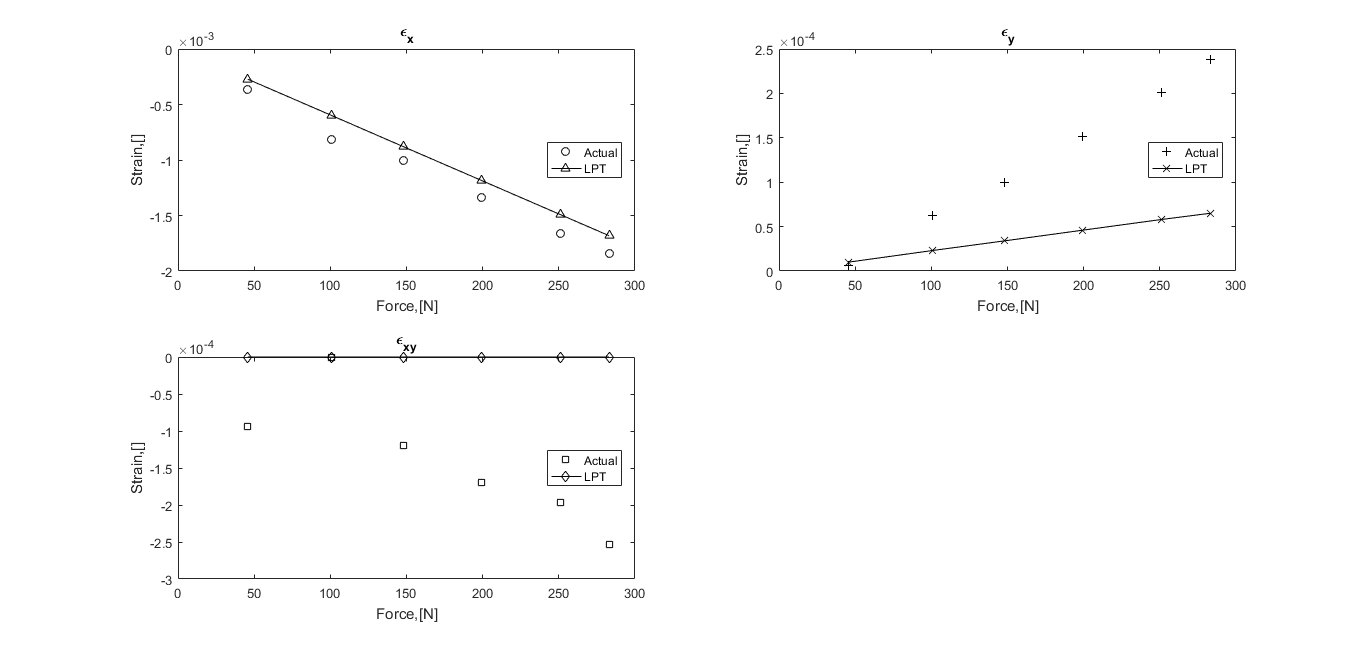
\includegraphics[width=1\textwidth]{FvsStrain.png}
	\caption{Force vs. Strain for Layup 3}
	\label{fig:FvStrain}
\end{figure}
% Test fixtures
\begin{figure}[H]
\centering
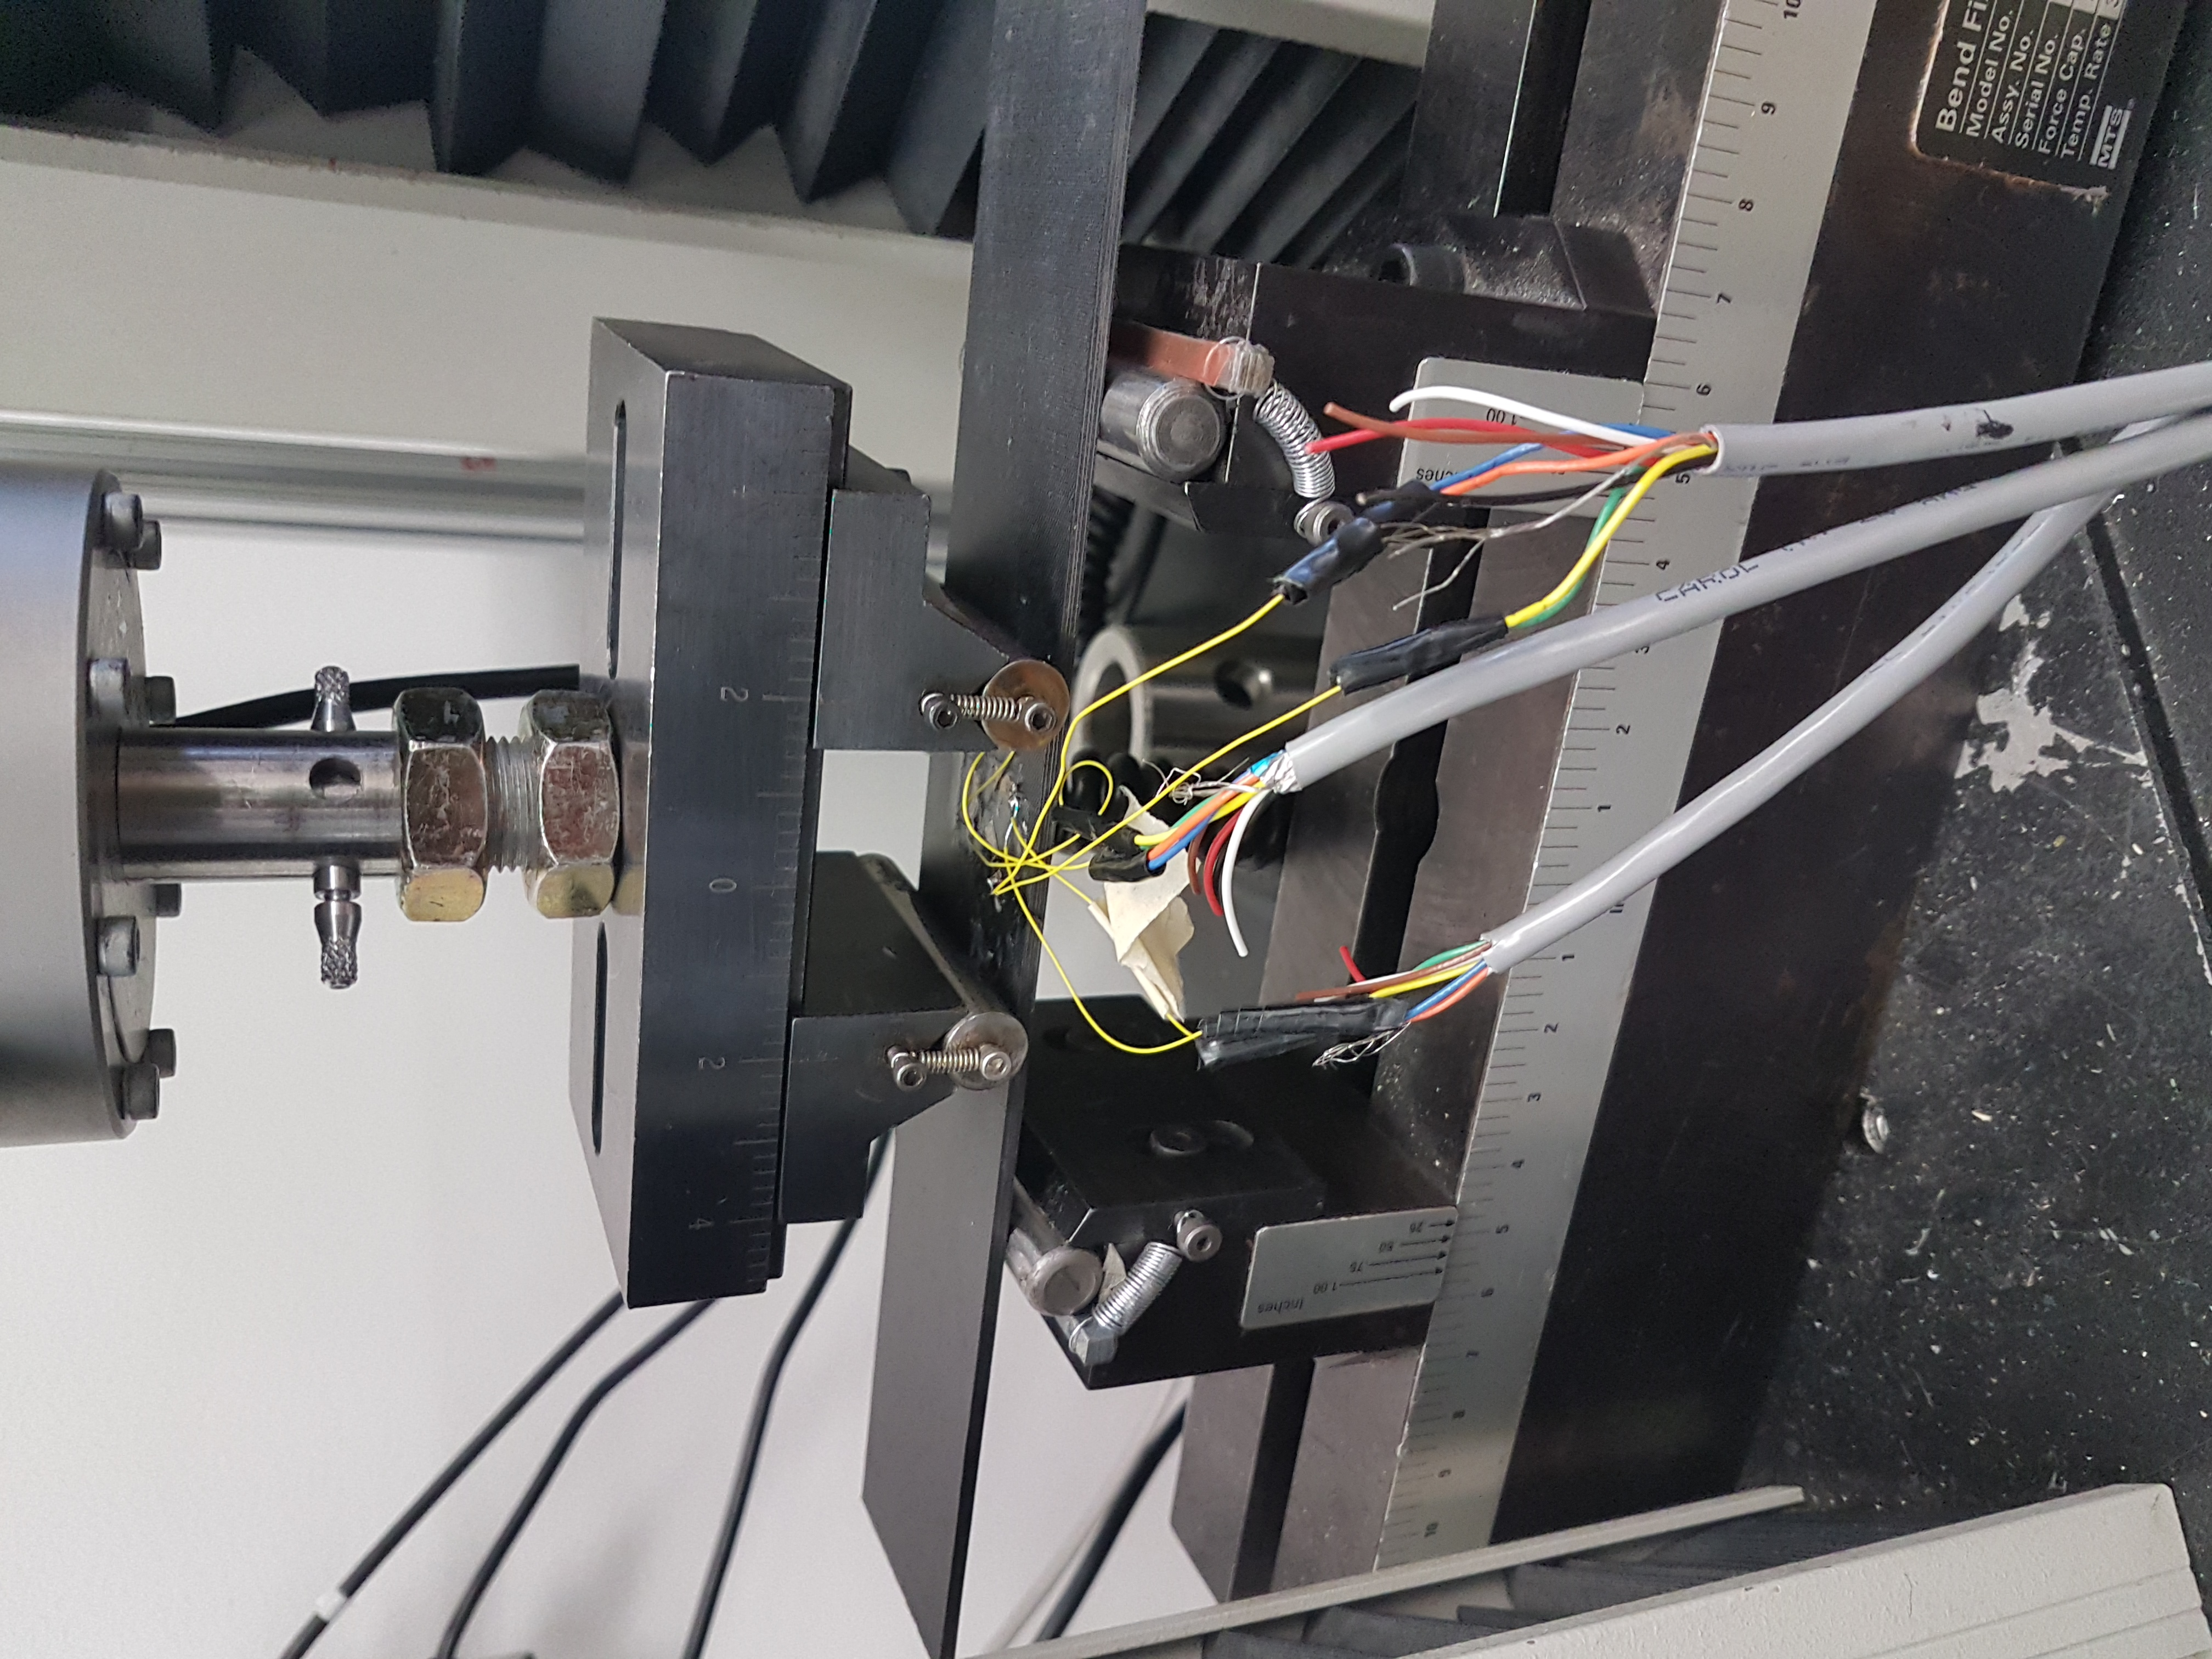
\includegraphics[width=0.8\textwidth]{fixture4pt.jpg}
\caption{Mechanical test set up with four-point bend fixture}
\label{fig:Fixture}
\end{figure}
% Moment Diagram
\begin{figure}[H]
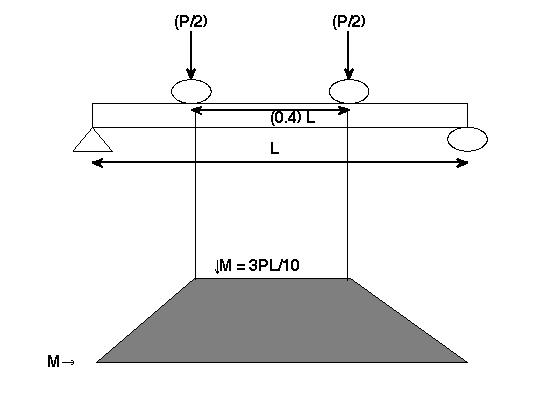
\includegraphics[width=0.8\textwidth]{4ptMomentDiagram.jpg}\label{fig:Mdiagram}
\caption{Moment diagram of four-point flexure setup used in mechincal testing.}
\end{figure}

% Specimen with gauge orientations
% Side view with layup
\section{Tables}
%Material Properties:
\begin{table}[h]\footnotesize
	\centering
	\begin{tabular}{ |l|l|l|l|l|l| }
		\hline
		Parameter&$\mathbf{E_1}$& $\mathbf{E_2}$ & $\mathbf{G_{12}}$ & $\mathbf{\nu_{12}}$ & $\mathbf{\nu_{21}}$ \\ \hline
		Value& 114 GPa & 8.3 GPa& 3.93 GPa &0.33 & 0.02\\ \hline
	\end{tabular}
	\caption{T800-3900 Material Properties}
	\label{tab:Material Properties}%
\end{table}
% All layups
\begin{table}[h]
	\centering
	\begin{tabular}{cc}
		Layup \# & Ply Orientation \\
		\midrule
		\midrule
		1     &$ [(90/45/0/45)_2]_S$ \\
		2     &$ [45/90]_4$ \\
		3     &$ [(90)_2/(0)_4/(90)_2]_S$ \\
		4     &$ [90/45/0/-45]_4$ \\
		5     &$ [(90)_2/(0)_2]_2$ \\
	\end{tabular}%
	\caption{Ply Orientation of Five Potential Layups}
    \label{tab:Ply}%
\end{table}%
%Raw Data:
\begin{table} [h]
	\centering
	\begin{tabular}{ccccrr}
		\multicolumn{2}{c}{Specimen Data} &       & \multicolumn{2}{c}{Strain Gage Data} &  \\
		\cmidrule{1-2}\cmidrule{4-5}    \multicolumn{1}{r}{Support Span:} & \multicolumn{1}{r}{0.127} & \multicolumn{1}{l}{(m)} & \multicolumn{1}{r}{Gage 1 Orientation:} & 90    & \multicolumn{1}{l}{(degrees)} \\
		\multicolumn{1}{r}{Load Span:} & \multicolumn{1}{r}{0.0508} & \multicolumn{1}{l}{(m)} & \multicolumn{1}{r}{Gage 2 Orientation:} & 0     & \multicolumn{1}{l}{(degrees)} \\
		\multicolumn{1}{r}{Length:} & \multicolumn{1}{r}{0.305} & \multicolumn{1}{l}{(m)} & \multicolumn{1}{r}{Gage 3 Orientation:} & 45    & \multicolumn{1}{l}{(degrees)} \\
		\multicolumn{1}{r}{Width:} & \multicolumn{1}{r}{0.04925} & \multicolumn{1}{l}{(m)} &       &       &  \\
		\multicolumn{1}{r}{Thickness:} & \multicolumn{1}{r}{0.0028} & \multicolumn{1}{l}{(m)} & \multicolumn{1}{r}{Excitation Voltage:} & 12    & \multicolumn{1}{l}{(V)} \\
		&       &       & \multicolumn{1}{r}{Gage Factor:} & 2.125 &  \\
		&       &       & \multicolumn{1}{r}{Dewetron Setting:} & 83.333 & \multicolumn{1}{l}{(mv/V)} \\
		&       &       & \multicolumn{1}{r}{Calculated Gain:} & 5.00002 &  \\
		&       &       &       &       &  \\
		\multicolumn{4}{c}{Collected Load and Voltage Data} &       &  \\
		\cmidrule{1-4}    \multicolumn{4}{c}{Gages on Top:} &       &  \\
		Load (N) & Gage 1 Voltage & Gage 2 Voltage & Gage 3 Voltage &       &  \\
		45.78 & -0.0002 & 0.0116 & 0.0072 &       &  \\
		100.5 & -0.002 & 0.026 & 0.012 &       &  \\
		148.3 & -0.0032 & 0.0322 & 0.0164 &       &  \\
		199.5 & -0.0048 & 0.0426 & 0.0216 &       &  \\
		251   & -0.0064 & 0.053 & 0.0264 &       &  \\
		283   & -0.0076 & 0.0588 & 0.0296 &       &  \\
		&       &       &       &       &  \\
		\multicolumn{4}{c}{Gages on Bottom:} &       &  \\
		Load (N) & Gage 1 Voltage & Gage 2 Voltage & Gage 3 Voltage &       &  \\
		55.98 & 0.0044 & -0.0092 & -0.0064 &       &  \\
		104.7 & 0.006 & -0.0196 & -0.0124 &       &  \\
		160.7 & 0.0072 & -0.0316 & -0.0196 &       &  \\
		204.8 & 0.0084 & -0.0396 & -0.0252 &       &  \\
		256.5 & 0.008 & -0.049 & -0.032 &       &  \\
		279.1 & 0.0104 & -0.053 & -0.0352 &       &  \\
	\end{tabular}%
	\caption{Measured Data From Experimental Process}
	\label{tab:Raw Data}%
\end{table}
% Layups strain LPT
\begin{table}[htbp]
	\centering
	\begin{tabular}{rrrrrrr}
		&       &       & \multicolumn{1}{l}{$\epsilon_x$} &       &       &  \\
		&       & \multicolumn{5}{c}{LPT Predicted} \\
		\cmidrule{3-7}    \multicolumn{1}{c}{Load (N)} & \multicolumn{1}{c}{Actual Strain} & \multicolumn{1}{c}{Layup 1} & \multicolumn{1}{c}{Layup 2} & \multicolumn{1}{c}{Layup 3} & \multicolumn{1}{c}{Layup 4} & \multicolumn{1}{c}{Layup 5} \\
		45.78 & -0.000364 & -0.000447 & -0.004975 & -0.000272 & -0.000345 & -0.001291 \\
		100.5 & -0.000815 & -0.000981 & -0.010920 & -0.000597 & -0.000758 & -0.002833 \\
		148.3 & -0.001009 & -0.001447 & -0.016110 & -0.000882 & -0.001118 & -0.004180 \\
		199.5 & -0.001335 & -0.001947 & -0.021680 & -0.001186 & -0.001504 & -0.005624 \\
		251   & -0.001660 & -0.002450 & -0.027280 & -0.001492 & -0.001893 & -0.007075 \\
		283   & -0.001841 & -0.002762 & -0.030750 & -0.001682 & -0.002134 & -0.007977 \\
		&       &       &       &       &       &  \\
		&       &       & \multicolumn{1}{l}{$\epsilon_y$} &       &       &  \\
		&       & \multicolumn{5}{c}{LPT Predicted} \\
		\cmidrule{3-7}    \multicolumn{1}{c}{Load (N)} & \multicolumn{1}{c}{Actual Strain} & \multicolumn{1}{c}{Layup 1} & \multicolumn{1}{c}{Layup 2} & \multicolumn{1}{c}{Layup 3} & \multicolumn{1}{c}{Layup 4} & \multicolumn{1}{c}{Layup 5} \\
		45.78 & 0.000006 & 0.000041 & 0.000418 & 0.000010 & 0.000092 & -0.000048 \\
		100.5 & 0.000063 & 0.000089 & 0.000918 & 0.000023 & 0.000203 & 0.000104 \\
		148.3 & 0.000100 & 0.000131 & 0.001354 & 0.000034 & 0.000299 & 0.000154 \\
		199.5 & 0.000151 & 0.000177 & 0.001822 & 0.000046 & 0.000403 & 0.000207 \\
		251   & 0.000201 & 0.000222 & 0.002292 & 0.000058 & 0.000507 & 0.000261 \\
		283   & 0.000238 & 0.000251 & 0.002584 & 0.000065 & 0.000571 & 0.000294 \\
		&       &       &       &       &       &  \\
		&       &       & \multicolumn{1}{l}{$\epsilon_{xy}$} &       &       &  \\
		&       & \multicolumn{5}{c}{LPT Predicted} \\
		\cmidrule{3-7}    \multicolumn{1}{c}{Load (N)} & \multicolumn{1}{c}{Actual Strain} & \multicolumn{1}{c}{Layup 1} & \multicolumn{1}{c}{Layup 2} & \multicolumn{1}{c}{Layup 3} & \multicolumn{1}{c}{Layup 4} & \multicolumn{1}{c}{Layup 5} \\
		45.78 & -0.000094 & 0.000308 & 0.003713 & 0.000000 & 0.000024 & 0.000000 \\
		100.5 & 0.000000 & 0.000675 & 0.008150 & 0.000000 & 0.000054 & 0.000000 \\
		148.3 & -0.000120 & 0.000996 & 0.012030 & 0.000000 & 0.000079 & 0.000000 \\
		199.5 & -0.000170 & 0.001340 & 0.016180 & 0.000000 & 0.000107 & 0.000000 \\
		251   & -0.000196 & 0.001686 & 0.020360 & 0.000000 & 0.000134 & 0.000000 \\
		283   & -0.000253 & 0.001901 & 0.022950 & 0.000000 & 0.000151 & 0.000000 \\
	\end{tabular}%
	\caption{Predicted vs. Actual Strain Values for Potential Layups}
	\label{tab:Strains}%
\end{table}%

\section{Appendix}

\subsection{Code}

\begin{verbatim}

% LPT Code
%Text inputs to inputs.txt
%Line 1 is material properties E1, E2, G12, v12
%Line 2 is strength for failure critereon
%Line 3 is thermal coefficients
%Line 4 is ply thickness
%Line 5 is ply orientation layup
%Line 6 is loading - N_x, N_y, N_xy, M_x, M_y, M_xy
%Line 7 is temperature change

clear, clc
format short g

F = csvread ('inputs.txt');
fileID = fopen('inputs.txt');
C = textscan(fileID,'%f %f %f %f %f %f %f %f %f %f %f %f %f %f %f %f %f %f %f %f %f %f %f %f %f %f','delimiter',',');
fclose(fileID);

for k = 1:length(C)
ply(k) = C{k}(5);
end
ply(find(isnan(ply))) = [];

% Name constants from text file:
% Material properties:
E1 = F(1,1);
E2 = F(1,2);
G = F(1,3);
v = F(1,4);

% Strength Properties:
S_L_plus = F(2,1);
S_L_minus = F(2,2);
S_T_plus = F(2,3);
S_T_minus = F(2,4);
S_LT = F(2,5);

% Coefficients of thermal expansion
alpha_1 = F(3,1);
alpha_2 = F(3,2);

% Ply thickness\
t = F(4,1);

% Laminate stacking
L = ply;

% Forces and moments
N_x = F(6,1);
N_y = F(6,2);
N_xy = F(6,3);
M_x = F(6,4);
M_y = F(6,5);
M_xy = F(6,6);

% Temperature change
Temp = F(7,1);

%1. Calculate Q and S matrices:

R = [1 0 0
0 1 0
0 0 2];

S = [1/E1 -v/E1 0
-v/E1 1/E2 0
0 0 1/G];

Q = inv(S);

% 1. Calculate Q_bar and S_bar matrices
for i = 1:length(L)
theta = L(i);

T = [(cosd(theta)).^2 (sind(theta)).^2 2*sind(theta).*cosd(theta)
(sind(theta)).^2 (cosd(theta)).^2 -2*sind(theta).*cosd(theta)
-sind(theta).*cosd(theta) sind(theta).*cosd(theta) (cosd(theta)).^2-(sind(theta)).^2];

Q_bar(:,(i*3-2):i*3) = T\Q*R*T/(R);
S_bar(:,(i*3-2):i*3) = inv(Q_bar(:,(i*3-2):i*3));

end

% Calculate Z values for plies:

for i= 1:length(L)+1
z(i) = -length(L)/2*t+((i-1)*t);
end

% 2. Calculate ABD matrix and inverse

A = zeros(3);
B = zeros(3);
D = zeros(3);
ABD = zeros(6);

for i= 1:3
for j= 1:length(L)
A(i,1) = A(i,1)+Q_bar(i,(j*3)-2)*(z(j+1)-z(j));
A(i,2) = A(i,2)+Q_bar(i,(j*3)-1)*(z(j+1)-z(j));
A(i,3) = A(i,3)+Q_bar(i,(j*3)-0)*(z(j+1)-z(j));
B(i,1) = B(i,1)+0.5*(Q_bar(i,(j*3)-2)*(z(j+1)^2-z(j)^2));
B(i,2) = B(i,2)+0.5*(Q_bar(i,(j*3)-1)*(z(j+1)^2-z(j)^2));
B(i,3) = B(i,3)+0.5*(Q_bar(i,(j*3)-0)*(z(j+1)^2-z(j)^2));
D(i,1) = D(i,1)+(1/3)*(Q_bar(i,(j*3)-2)*(z(j+1)^3-z(j)^3));
D(i,2) = D(i,2)+(1/3)*(Q_bar(i,(j*3)-1)*(z(j+1)^3-z(j)^3));
D(i,3) = D(i,3)+(1/3)*(Q_bar(i,(j*3)-0)*(z(j+1)^3-z(j)^3));
end
end

% make values 0 that should be 0:
for i= 1:3
for j= 1:3
if A(i,j) < 1*10^-12 && A(i,j) > -1*10^-12
A(i,j) = 0;
end
if B(i,j) < 1*10^-12 && B(i,j) > -1*10^-12
B(i,j) = 0;
end
if D(i,j) < 1*10^-12 && D(i,j) > -1*10^-12
D(i,j) = 0;
end
end
end

ABD(1:3,1:3) = A;
ABD(4:6,1:3) = B;
ABD(1:3,4:6) = B;
ABD(4:6,4:6) = D;
ABDinv = ABD^-1;

% 3. Apparent laminate stiffness properties:
E_x = 1/(length(L)*t*ABDinv(1,1));
E_y = 1/(length(L)*t*ABDinv(2,2));
v_xy = -ABDinv(1,2)/ABDinv(1,1);
G_xy = 1/(length(L)*t*ABDinv(3,3));
E_fx = 12/((length(L)*t)^3*ABDinv(4,4));
E_fy = 12/((length(L)*t)^3*ABDinv(5,5));

% 4. Midplane strains and curvatures
% Calculate thermal expansion coefficients in x-y:
% Calculate N and M thermal
alpha = [alpha_1,alpha_2,0]';
N_T = [0,0,0]';
M_T = [0,0,0]';
for i = 1:length(L)
theta = L(i);

T = [(cosd(theta)).^2 (sind(theta)).^2 2*sind(theta).*cosd(theta)
(sind(theta)).^2 (cosd(theta)).^2 -2*sind(theta).*cosd(theta)
-sind(theta).*cosd(theta) sind(theta).*cosd(theta) (cosd(theta)).^2-(sind(theta)).^2];
alpha_xy = inv(T)*alpha;
Q_bar_T = T\Q*R*T/(R);
N_T = N_T+Temp*Q_bar_T*alpha_xy*(z(i+1)-z(i));
M_T = M_T+0.5*Temp*Q_bar_T*alpha_xy*(z(i+1)^2-z(i)^2);
end
N = [N_x,N_y,N_xy]'+N_T;
M = [M_x,M_y,M_xy]'+M_T;
NM = [N
M];

strain_mid = ABDinv*NM;

eps_x_mid = strain_mid(1);
eps_y_mid = strain_mid(2);
eps_xy_mid = strain_mid(3);
K_x = strain_mid(4);
K_y = strain_mid(5);
K_xy = strain_mid(6);

% 5. Calculation of strains at all points in laminate and plot

% Calculation of mechanical strain
eps_mech_x = eps_x_mid + z*K_x;
eps_mech_y = eps_y_mid + z*K_y;
eps_mech_xy = eps_xy_mid + z*K_xy;

eps_mech = [eps_mech_x;eps_mech_y;eps_mech_xy];

figure(1)
plot(eps_mech_x,z,'r-',eps_mech_y,z,'b-',eps_mech_xy,z,'g-')
set(gca,'ydir','reverse')
legend('\epsilon_x','\epsilon_y','\epsilon_x_y')
grid on
xlabel('Strain, []')
ylabel('z,[m]')
title('Part 5 - Strain')

% 6. Calculation of stresses at top and bottom of ply:

% Get repeating z values at ply interfaces
for i=1:length(L)+1
zplot((i*2)-1)=z(i);
zplot(i*2)=z(i);
end
zplot(2*(length(L)+1)) = [];
zplot(1) = [];


for i = 1:length(L)
theta = L(i);
T = [(cosd(theta)).^2 (sind(theta)).^2 2*sind(theta).*cosd(theta)
(sind(theta)).^2 (cosd(theta)).^2 -2*sind(theta).*cosd(theta)
-sind(theta).*cosd(theta) sind(theta).*cosd(theta) (cosd(theta)).^2-(sind(theta)).^2];
alpha_xy = inv(T)*alpha;
eps_therm = alpha_xy*Temp;
eps1 = eps_mech(:,i)-eps_therm;
eps2 = eps_mech(:,i+1)-eps_therm;
stress_top(:,i) = Q_bar(:,3*i-2:3*i)*(eps1);
stress_bottom(:,i) = Q_bar(:,3*i-2:3*i)*(eps2);
end

for i = 1:length(L)
stress_xy(:,i*2-1) = stress_top(:,i);
stress_xy(:,i*2) = stress_bottom(:,i);
end

% 7. Plots of global stresses for each ply:

figure(2)
plot(stress_xy(1,:),zplot,'-*')
legend('\sigma_x')
set(gca,'ydir','reverse')
grid on
xlabel('\sigma_x,[Pa]')
ylabel('z,[m]')
title('\sigma_x')

figure(3)
plot(stress_xy(2,:),zplot,'-*')
legend('\sigma_y')
set(gca,'ydir','reverse')
grid on
xlabel('\sigma_y, [Pa]')
ylabel('z,[m]')
title('\sigma_y')

figure(4)
plot(stress_xy(3,:),zplot,'-*')
legend('\sigma_x_y')
set(gca,'ydir','reverse')
grid on
xlabel('\sigma_x_y,[Pa]')
ylabel('z, [m]')
title('\sigma_x_y')

% 8. Material coordinates on top and bottom of each ply

for i = 1:length(L)
theta = L(i);

T = [(cosd(theta)).^2 (sind(theta)).^2 2*sind(theta).*cosd(theta)
(sind(theta)).^2 (cosd(theta)).^2 -2*sind(theta).*cosd(theta)
-sind(theta).*cosd(theta) sind(theta).*cosd(theta) (cosd(theta)).^2-(sind(theta)).^2];

alpha_xy = inv(T)*alpha;
eps_therm = alpha_xy*Temp;
eps1 = eps_mech(:,i)-eps_therm;
eps2 = eps_mech(:,i+1)-eps_therm;
stress_top(:,i) = Q_bar(:,3*i-2:3*i)*(eps1);
stress_bottom(:,i) = Q_bar(:,3*i-2:3*i)*(eps2);
stress_top_12(:,i) = T*stress_top(:,i);
stress_bottom_12(:,i) = T*stress_bottom(:,i);
end

for i = 1:length(L)
stress_12(:,i*2-1) = stress_top_12(:,i);
stress_12(:,i*2) = stress_bottom_12(:,i);
end

% 9. Hashin Failure Criteria:

Fiber_Failure = ((stress_12(1,:).^2)./(S_L_plus*S_L_minus))+...
((1/S_L_plus-1/S_L_minus).*stress_12(1,:))+...
((stress_12(3,:).^2)./(S_LT^2));
Resin_Failure = ((stress_12(2,:).^2)./(S_T_plus*S_T_minus))+...
((1/S_T_plus-1/S_T_minus).*stress_12(2,:))+...
((stress_12(3,:).^2)./(S_LT^2));

mode = 'No Failure';
M=0;

i = 1;
while i <= length(L)
theta2((i*2)-1)=L(i);
theta2(i*2)=L(i);
i = i+1;
end

if max(Fiber_Failure) >= 1
mode = 'Fiber Failure';
[M, I] = max(Fiber_Failure);
z_fail_f = zplot(I);
ply_fail_f = theta2(I);
end
if max(Resin_Failure) >= 1
[M2, I2] = max(Resin_Failure);
if M2 > M
mode = 'Resin Failure';
z_fail_r = zplot(I2);
ply_fail_r = theta2(I2);
end
end

% Outputs to .txt file:
i = 1;
fid = fopen( 'outputs_JohnCallaway.txt', 'wt' );
fprintf(fid,'John Callaway \n');
fprintf(fid,'LPT Code - Spring 2017 \n');
fprintf(fid,'\n Part 1 \n');
for i = 1:length(L)
fprintf(fid,'\n Ply %i: \n',i);
fprintf(fid,'\n The Q matrix is:\n');
fprintf(fid,'%8.3g %8.3g %8.3g\n',Q);
fprintf(fid,'\n The Q bar Matrix is:\n');
fprintf(fid,'%8.3g %8.3g %8.3g\n',Q_bar(:,i*3-2:i*3));
fprintf(fid,'\n The S matrix is:\n');
fprintf(fid,'%8.3g %8.3g %8.3g\n',S);
fprintf(fid,'\n The S bar Matrix is:\n');
fprintf(fid,'%8.3g %8.3g %8.3g\n',S_bar(:,i*3-2:i*3));
end
fprintf(fid,'\n Part 2: \n');
fprintf(fid,'\n The ABD matrix is: \n');
fprintf(fid,'%8.4g %8.4g %8.4g %8.4g %8.4g %8.4g \n',ABD);
fprintf(fid,'\n The ABD inverse matrix is: \n');
fprintf(fid,'%8.4g %8.4g %8.4g %8.4g %8.4g %8.4g \n',ABDinv);

fprintf(fid,'\n Part 3: \n');
fprintf(fid,'\n E_x is: \n');
fprintf(fid,'%8.2g \n', E_x);
fprintf(fid,'\n E_y is: \n');
fprintf(fid,'%8.2g \n', E_y);
fprintf(fid,'\n v_xy is: \n');
fprintf(fid,'%8.2g \n', v_xy);
fprintf(fid,'\n G_xy is: \n');
fprintf(fid,'%8.2g \n', G_xy);
fprintf(fid,'\n E_fx is: \n');
fprintf(fid,'%8.2g \n', E_fx);
fprintf(fid,'\n E_fy is: \n');
fprintf(fid,'%8.2g \n', E_fy);

fprintf(fid,'\n Part 4: \n');
fprintf(fid,'\n Midplane Strain in x is: \n');
fprintf(fid,'%8.4g \n',eps_x_mid);
fprintf(fid,'\n Midplane Strain in y is: \n');
fprintf(fid,'%8.4g \n',eps_y_mid);
fprintf(fid,'\n Midplane Strain in xy is: \n');
fprintf(fid,'%8.4g \n',eps_xy_mid);
fprintf(fid,'\n Curvature in x is: \n');
fprintf(fid,'%8.4g \n',K_x);
fprintf(fid,'\n Curvature in y is: \n');
fprintf(fid,'%8.4g \n',K_y);
fprintf(fid,'\n Curvature in xy is: \n');
fprintf(fid,'%8.4g \n',K_xy);

fprintf(fid,'\n Part 6: \n');
fprintf(fid,'\n Global Coordinate Stresses: \n');
for i = 1:length(L)
fprintf(fid,'\n Ply %i Top:',i); 
fprintf(fid,' %8.4g %8.4g %8.4g \n',stress_top(:,i));
fprintf(fid,'\n Ply %i Bottom:',i); 
fprintf(fid,' %8.4g %8.4g %8.4g \n',stress_bottom(:,i));
end

fprintf(fid,'\n Part 8: \n');
fprintf(fid,'\n Material Coordinate Stresses: \n');
for i = 1:length(L)
fprintf(fid,'\n Ply %i Top:',i); 
fprintf(fid,' %8.4g %8.4g %8.4g \n',stress_top_12(:,i));
fprintf(fid,'\n Ply %i Bottom:',i); 
fprintf(fid,' %8.4g %8.4g %8.4g \n',stress_bottom_12(:,i));
end

fprintf(fid,'\n Part 9: \n');

if strcmp(mode,'No Failure')
fprintf(fid,'\n No failure occured \n');
end
if strcmp(mode,'Fiber Failure')
fprintf(fid,'Ply %i failed first, its orientation is %d degrees \n',ceil(I/2),ply_fail_f);
fprintf(fid,'The location of the failure is %8.3g m \n',z_fail_f');
fprintf(fid,'The failure occured in the fibers \n');
end
if strcmp(mode,'Resin Failure')
fprintf(fid, 'Ply %i failed first, its orientation is %d degrees \n',ceil(I2/2),ply_fail_r);
fprintf(fid, 'The location of the failure is %8.3g m \n',z_fail_r');
fprintf(fid, 'The failure occured in the resin \n');
end
\end{verbatim}

\subsection{equations}


\begin{equation}
[Q]=\left[\begin{matrix}
\frac{E_1}{1-\nu_{12}\nu{21}}&\frac{\nu_{12}E_2}{1-\nu_{12}\nu{21}}&0\\
\frac{\nu_{12}E_2}{1-\nu_{12}\nu{21}}&\frac{E_2}{1-\nu_{12}\nu{21}}&0\\
0&0&\frac{1}{G_{12}}\\
\end{matrix}\right]
\end{equation}

\begin{equation}
[T]=\left[\begin{matrix}
\cos^2(\theta)& \sin^2(\theta) & 2\sin(\theta)\cos(\theta)\\
 \sin^2(\theta) & \cos^2(\theta)& -2\sin(\theta)\cos(\theta)\\
 -\sin(\theta)\cos(\theta)&\sin(\theta)\cos(\theta)&\cos^2(\theta)-sin^2(\theta)
\end{matrix}\right]
\end{equation}
\begin{equation}
[R]=\left[\begin{matrix}
1 & 0 & 0\\ 0 & 1 & 0\\ 0& 0 &2
\end{matrix}\right]
\end{equation}
\\ \\
\begin{equation}
\bar{Q}=T^{-1} Q R T R^{-1}
\end{equation}

\begin{align}
A_{ij}&=\sum_{k=1}^{N}\left(\bar{Q_{ij}}\right)_k(z_{k}-z_{k-1})\\
B_{ij}&=\sum_{k=1}^{N}\left(\bar{Q_{ij}}\right)_k(z_{k}^2-z_{k-1}^2)\\
D_{ij}&=\sum_{k=1}^{N}\left(\bar{Q_{ij}}\right)_k(z_{k}^3-z_{k-1}^3)
\end{align}

\begin{equation}
\left[\begin{matrix}
N_{x}\\ N_{y} \\ N_{xy} \\ M_{x} \\ M_{y} \\ M_{xy}
\end{matrix}\right] = \left[\begin{matrix}
A_{11} & A_{12} & A_{16} & B__{11} & B_{12} & B_{16} \\ 
A_{21} & A_{22} & A_{26} & B__{21} & B_{22} & B_{26} \\
A_{61} & A_{62} & A_{66} & B__{61} & B_{62} & B_{66} \\
B_{11} & B_{12} & B_{16} & D__{11} & D_{12} & D_{16} \\
B_{21} & B_{22} & B_{26} & D__{21} & D_{22} & D_{26} \\
B_{61} & B_{62} & B_{66} & D__{61} & D_{62} & D_{66}
\end{matrix}\right] \left[\begin{matrix}
\epsilon_{x}\\ \epsilon_{y} \\ \epsilon_{xy} \\ \kappa_{x} \\ \kappa_{y} \\ \kappa_{xy} 
\end{matrix}\right]
\end{equation}

% 45 rossete
 \begin{equation}
 \gamma_{xy} = 2\epsilon_{OB} -(\epsilon_{x}+\epsilon_{y})\label{eq:45Rosette}
\end{equation}
%voltage to strain
\begin{equation}
\epsilon =\frac{-2V_{r}}{GF[(v+1)-V_{r}(v - 1)]}\label{eq:Ve}
\end{equation}
\begin{equation}
%voltage ratio
V_{R} = \frac{V_{CH}-V_{0}}{V_{EX} Gain}\label{eq:Vr}
\end{equation}
% gain
\begin{equation}
Gain = \frac{5}{(\frac{V_{EX}}{1000}){R_{shunt}}}\label{eq:gain}
\end{equation}
\begin{equation}
M = \frac{3PL}{10}\label{eq:moment}
\end{equation}


\bibliographystyle{IEEEtran}
\bibliography{Lab1Bib}
\end{document}